\documentclass[fleqn,12pt]{wlscirep}

\usepackage{verbatim}
\usepackage[superscript]{cite}
\usepackage{hyperref}
\usepackage{setspace}
\usepackage[singlelinecheck=false]{caption}

\pagenumbering{arabic}

\title{Shining a Light on Prokaryotic Bioluminescence Pathways:
A Comparative Genomics Approach}

\author[1,+]{Fotini (Tina) Papazotos}
\author[1,+]{Mathias Renaud}
\author[1,+]{Nicole Wang}
\author[1,+]{Debra Watkins}
\affil[1]{University of Waterloo, Dept. of Biology, Waterloo, Canada}
\affil[+]{these authors contributed equally to this work}

\begin{document}
\NoHyper
\flushbottom
\maketitle
\doublespace

\section*{Introduction}

Distinct groups of prokaryotes and eukaryotes are capable of bioluminescence, a process which allows an organism to emit light through enzymatic activity\cite{1}. Luciferase is the collective name for enzymes central to bioluminescence, which are capable of catalyzing visible light production, most commonly using luciferin as a substrate\cite{1,2}. Chemiluminescence pathways, including bioluminescence, differ from fluorescent proteins, such as GFP, because they do not require incoming light to luminesce\cite{3}. Though the specific enzymatic reactions differ, bioluminescence pathways are present in distantly related organisms across the different domains of life\cite{4}. This ability is typically found in marine or host-associated environments, but free-living bioluminescent freshwater and terrestrial prokaryotes have also been isolated\cite{4}.

The luciferase enzyme is commonly used in the fields of biotechnology, microscopy and in molecular biology, where it functions as a reporter gene\cite{6}. In these applications, luciferase acts similarly to GFP, but only requires the substrate luciferin and ATP to be detected, instead of an external light source\cite{7}. Luciferase is also used in next-generation 454 pyrosequencing, where the emitted light is an indicator of nucleotide incorporation to a growing nucleotide chain\cite{8}.

Bioluminescence is not fully understood, but is thought to play roles in evading predators, detecting and luring prey, sexual selection, and quorum sensing\cite{5}. Common bacterial genera that perform bioluminescence include \textit{Vibrio}, \textit{Aliivibrio}, \textit{Photobacterium}, and \textit{Photorhabdus}. The \textit{luxCDAB(F)E} operon is the common organization of \textit{lux} genes in most bacteria\cite{9}. \textit{luxA} and \textit{luxB} encode the subunits of heterodimeric luciferase protein\cite{9}. \textit{luxCDE} genes code for subunits of a fatty acid reductase protein, which synthesizes aldehyde substrates that drive the bioluminescence reaction\cite{9}. There are also other \textit{lux} genes that are generally not part of the \textit{lux} operon. \textit{luxI} and \textit{luxR} encode proteins that regulate expression of the \textit{lux} operon\cite{10}. \textit{luxF}, which is found in the \textit{lux} operon of some Photobacterium species, encodes flavoprotein\cite{10}. \textit{luxG} encodes a protein which acts as a flavin reductase producing FMNH2 , a substrate required for the reaction\cite{10}. Other \textit{lux} genes include \textit{luxPQNUO} which are not found in the operon\cite{11}.

\textit{luxS} encodes the protein S-ribosylhomocysteine lyase, which plays a role in the biosynthesis of a molecule involved in signaling cell density to other members of a bacterial population\cite{12}. Quorum sensing is an energy-conserving adaptation in which cells only expend the energy to express certain genes when the population density surpasses a threshold\cite{13}. This gene is therefore common among both bioluminescent and non-bioluminescent bacterial species.

\section*{Objectives}

The goal of this project was to compare the genomes of prokaryotic organisms which exhibit bioluminescence or contain genes included in the pathway, and to investigate whether this parallels phylogenetic relationships between these species.

It was hypothesized that there would be homology between the pathways responsible for bioluminescence in closely related prokaryotes. It was also hypothesized that the phylogenetic relationships of the organisms would parallel the relationships between bioluminescence pathways. 

\section*{Methods}

The sample of species for this project was selected from prokaryotes that have been previously identified in the literature as able to perform bioluminescence. \textit{E. coli} was included as an out group for these analyses since it is well studied, does not perform bioluminescence, and contains only one of the \textit{lux} genes, \textit{luxS}. For the 22 selected species, genome assemblies were downloaded from Ensembl and NCBI Assembly. A breakdown of these species is shown in table \ref{table1}.

% Table 1 %
\begin{table}[!ht]
\caption{Sample of Prokaryotic Species}
\begin{tabular}{llrrl}
Species Name                     & Accession Number  & Length & N50 & Environment        \\ \hline
\textit{Aliivibrio fischeri}              & ASM1180v1         & 4,273,718            & 2,897,536  & Marine, Symbiont \cite{21}   \\
\textit{Aliivibrio logei}                 & ASM169105v1       & 4,638,003            & 302,500    & Symbiont \cite{21}           \\
\textit{Aliivibrio salmonicida}           & ASM19649v1        & 4,655,660            & 3,325,165  & Symbiont \cite{22}           \\
\textit{Aliivibrio wodanis}               & AWOD1             & 4,635,126            & 3,003,353  & Symbiont \cite{4}            \\
\textit{Escherichia coli} (K12)           & ASM584v2          & 4,641,652            & 4,641,652  & Symbiont \cite{23}    \\
\textit{Photobacterium aquimaris}         & ASM167607v1       & 4,382,175            & 177,782    & Marine \cite{4}              \\
\textit{Photobacterium damselae}          & ASM167614v1       & 4,457,113            & 176,840    & Symbiont \cite{4}            \\
\textit{Photobacterium kishitanii}        & CFSAN029432\_01.0 & 4,709,666            & 174,214    & Symbiont \cite{21}           \\
\textit{Photobacterium leiognathi}        & CFSAN029437\_01.0 & 4,607,317            & 87,333     & Marine, Symbiont \cite{21}   \\
\textit{Photobacterium phosphoreum}       & CFSAN029438\_01.0 & 4,475,676            & 83,930     & Symbiont \cite{21}           \\
\textit{Candidatus Photodesmus katoptron} & ASM47868v1        & 1,015,921            & 555,626    & Marine, symbiont \cite{24}   \\
\textit{Photorhabdus asymbiotica}         & ASM19647v1        & 5,094,138            & 5,064,808  & Symbiont \cite{4}            \\
\textit{Photorhabdus luminescens}         & GCA\_000767775.1  & 5,596,724            & 186,732    & Symbiont \cite{4}            \\
\textit{Shewanella woodyi}                & ASM1952v1         & 5,935,403            & 5,935,403  & Marine, Symbiont \cite{4}    \\
\textit{Vibrio azureus}                   & ASM46716v1        & 4,716,275            & 60,692     & Marine \cite{25}             \\
\textit{Vibrio campbellii}                & ASM77265v1        & 5,652,224            & 947,033    & Marine \cite{26}             \\
\textit{Vibrio cholerae}                  & GFC\_11           & 4,012,216            & 80,785     & Freshwater, Marine \cite{21} \\
\textit{Vibrio harveyi}                   & ASM83407v1        & 5,864,537            & 162,233    & Marine, Symbiont \cite{21}   \\
\textit{Vibrio mediterranea}              & ASM235813v1       & 5,945,836            & 246,425    & Marine \cite{27}             \\
\textit{Vibrio orientalis}                & ASM17623v1        & 4,698,244            & 2,361,996  & Marine \cite{21}             \\
\textit{Vibrio sagamiensis}               & ASM40042v1        & 4,557,580            & 50,295     & Marine \cite{28}             \\
\textit{Vibrio splendidus}                & ASM130621v1       & 5,895,444            & 96,546     & Marine \cite{22}            
\end{tabular}
\\
\begin{flushleft}Prokaryotic species used for comparative genome analysis of bioluminescence pathway. The quality of each individual genome assembly was determined by comparing genome length to the N50 value.\end{flushleft}
\label{table1}
\end{table}

	An initial phylogenetic tree of the species was created using the online tool phyloT, which uses NCBI taxonomy to generate trees\cite{14}. The Newick tree file was visualized using Archaeopteryx, a java-based tool for visualizing phylogenetic trees\cite{15}.
    
	Each genome assembly was processed through the Prokka annotation pipeline. Prokka takes in assembled bacterial genomes in FASTA format and runs five different annotation programs on the sequences\cite{16}. The main program of interest to this study was Prodigal, which annotates protein coding sequences (CDSs)\cite{17}. The protein multi-FASTA output file (.faa) generated by Prodigal was used as the input for further analysis. This file contains each of the predicted CDSs. Additionally, the Genbank files (.gbk) were used for synteny analysis in Mauve in order to incorporate annotations into the aligned genomes.
    
	The protein multi-FASTA file for each species was run though the pfastGO pipeline. This pipeline is primarily for annotating bacterial protein sequences with GO terms. The input is a protein multi-FASTA file, which is used to perform BLASTp against Swiss-Prot to find homologs to the CDSs. PfamScan is also employed to search for conserved protein domains that may not have known homologs. The results from these two searches are used to transfer homology, GO terms, and KEGG IDs to each of the CDSs\cite{18}. Over 9 million homologs across the 22 genomes were narrowed down to just under 5000 by constraining to genes named “lux” found within the same genus as the query species.
    
	To look at differences in the complete sets of GO terms between the species, eggNog-mapper was used on the genome assemblies. This web-based tool provides the frequency of each GO term in a genome\cite{19}. The two heat maps for the \textit{lux} gene and GO term tables were generated in R using the heatmap.2 function from the gplots package.
    
	Lastly, a synteny analysis was done using Mauve. Mauve allows for alignment of multiple genomes, which was used to compare differences in \textit{lux} operon structure between the genera\cite{20}. All scripts and data used for this project can be found at \url{github.com/MathiasRenaud/BIOL469-Project}.


\section*{Results \& Discussion}

% Discussion %
Literature searches were performed to identify genes involved in the bioluminescence pathways of both prokaryotic and eukaryotic species. A preliminary comparison of the amino acid sequences of eukaryotic and prokaryotic luciferase proteins was then conducted using Blastp searches. These Blastp results, shown in table \ref{table2}, yielded low sequence identity and high E-values, indicating that bioluminescence pathways of prokaryotes and eukaryotes are likely not homologous, and possibly arose by convergent evolution. Due to the low similarity observed between prokaryotic and eukaryotic luciferase proteins, only bacterial bioluminescence genes were analyzed in this project.\\

% Table 2 %
\begin{table}[!ht]
\caption{Comparison of Eukaryote and Prokaryote Luciferases}
\resizebox{\textwidth}{!}{\begin{tabular}{llrr}
Eukaryotic Protein                   & Bacterial Protein                                           & Sequence Identity & E value \\ \hline
Fire Fly Luciferase (Q27758)         & \textit{V.harveyi} (\textit{LuxA}) Luciferase alpha subunit (B2XS31)          & 38\%        & 8.3     \\
Dinoflagellate Luciferase (O77206)   & \textit{Photobacterium phosphoreum} Beta luciferase subunit (Q52099) & 26\%        & 2       \\
\textit{Photinus pyralis} Luciferase (A3KBZ8) & \textit{Vibrio campbellii} (\textit{LuxB}) Luciferase subunit B (A8JPA2)      & 26\%        & 0.69   
\end{tabular}}
\\
\begin{flushleft}Preliminary comparison of prokaryotic and eukaryotic luciferase genes. Conducted using Blastp, to find sequence identity and E values between representative prokaryotic and eukaryotic luciferases.\end{flushleft}
\label{table2}
\end{table}

% KEGG Pathways %
\begin{figure}[ht]
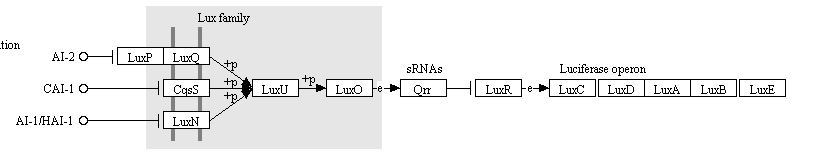
\includegraphics[width=\textwidth]{pathway-1.png}
\caption{The Kegg Pathway of two-component system by the \textit{lux} family.\cite{11}}
\centering
\label{fig5}
\end{figure}

\begin{figure}[ht]
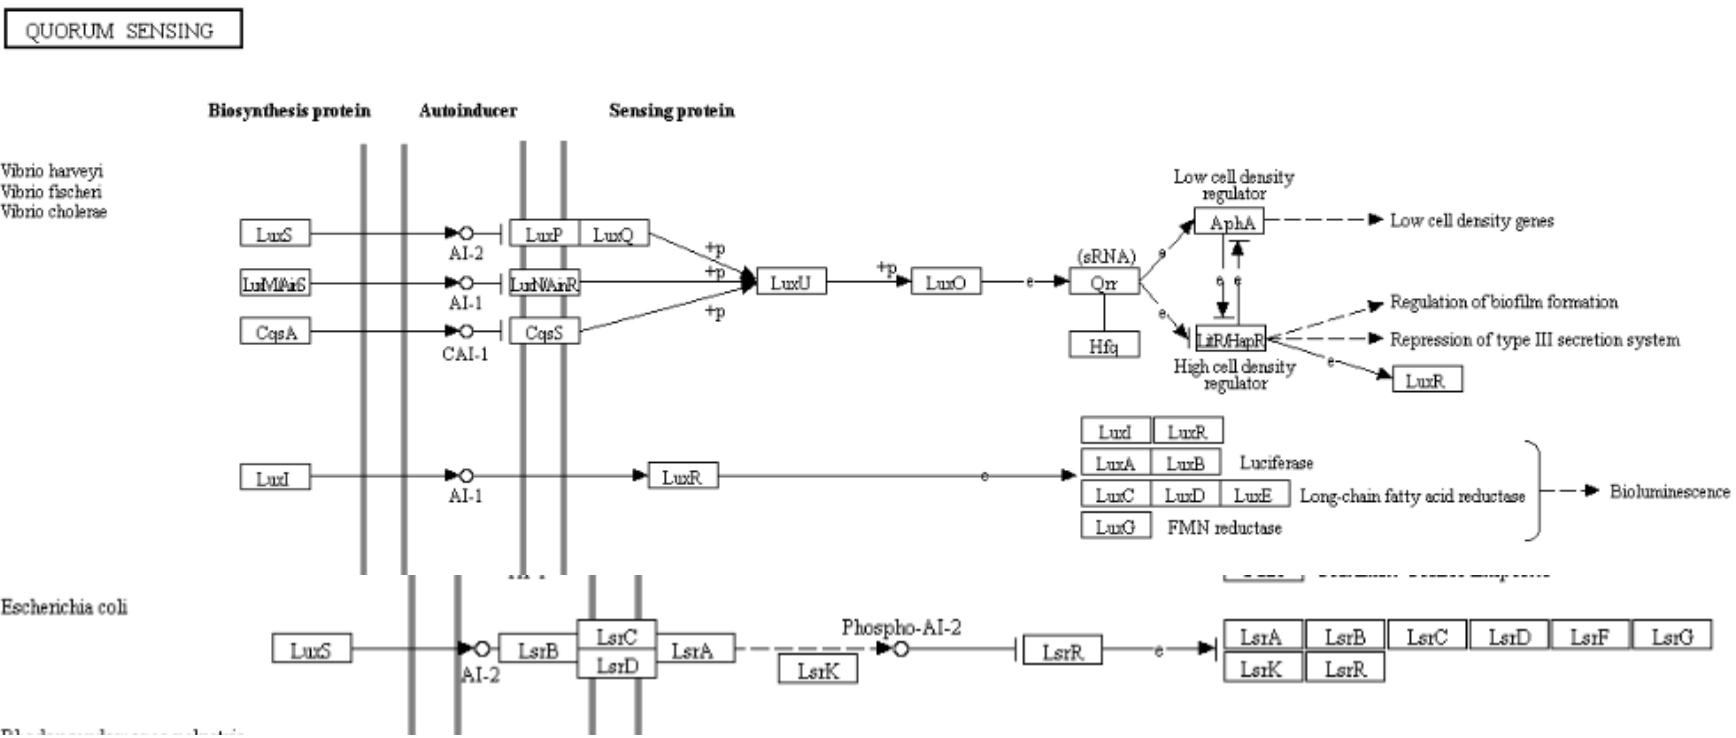
\includegraphics[width=\textwidth]{pathway-2.png}
\caption{The KEGG Pathway of Quorum Sensing by the \textit{lux} family.\cite{11}}
\centering
\label{fig6}
\end{figure}

22 bacteria were chosen to be analyzed based on a literature search of prokaryotes that exhibit bioluminescence. Several common genera were found to carry out the light-producing pathway, including \textit{Vibrio}, \textit{Aliivibrio}, \textit{Photobacterium}, and \textit{Photorhabdus}. Two pathways were found to be associated with luciferases upon a KEGG Pathway database search: a two-component regulatory pathway (figure \ref{fig5}), and a quorum sensing pathway (figure \ref{fig6})\cite{d7}. Both pathways were further investigated and it was found that the two-component system involving the luciferase family plays a role in regulation of the quorum sensing pathways \cite{d1}. 

\begin{figure}[ht]
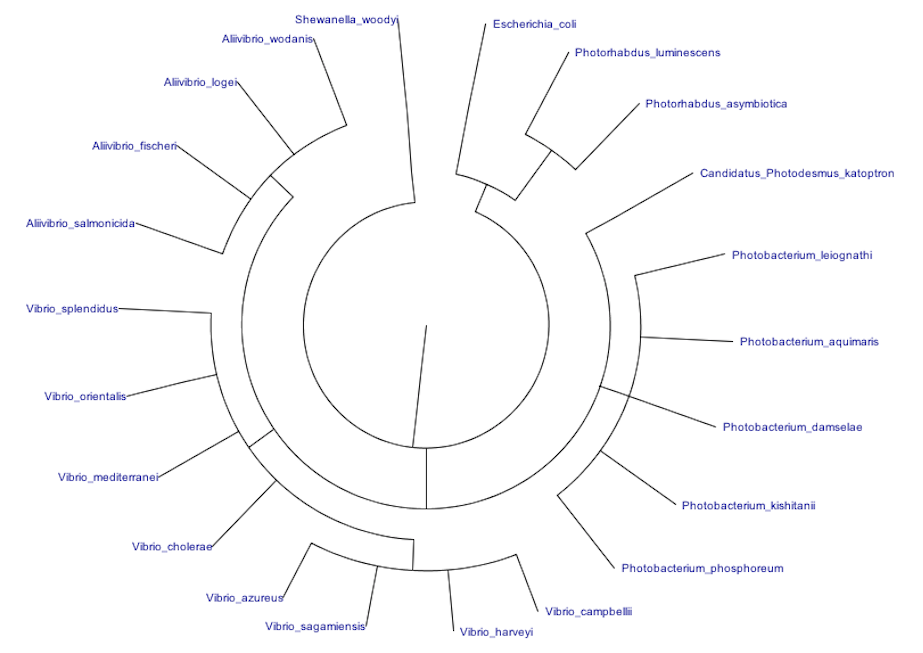
\includegraphics[width=\textwidth]{1.png}
\caption{Phylogenetic tree derived from NCBI taxonomy. \textit{E. coli} was included in the analysis as an outgroup, but was actually determined to cluster with \textit{Photorhabdus}. The phyloT tree building program was used to develop the tree based on NCBI taxonomy.}
\centering
\label{fig1}
\end{figure}

To examine relationships between bioluminescent species, a phylogenetic tree of the 22 chosen bacterial genomes was computed based on NCBI taxonomy. This tree was then used to compare against the functional relationships between these same species. Figure \ref{fig1} shows the phylogenetic tree based on NCBI taxonomy. In this phylogeny-based tree, \textit{S. woodyi} was an outgroup.

\begin{figure}[ht]
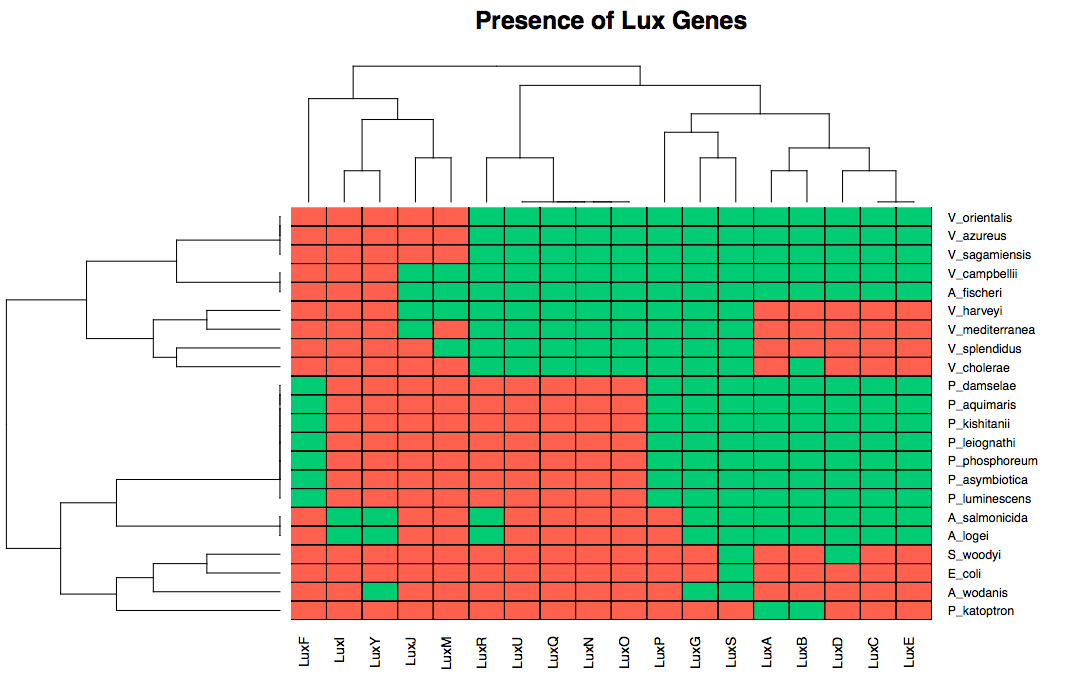
\includegraphics[width=\textwidth]{2.png}
\caption{Plotting the presence of \textit{lux} genes in bacteria. For each bacterial species, any \textit{lux} gene present in their genome is coloured green, and the \textit{lux} genes absent are coloured red. The 22 bacteria are also clustered into a tree based on their \textit{lux} gene sets (B).}
\centering
\label{fig2}
\end{figure}

The \textit{lux} gene heatmap in figure \ref{fig2} shows the presence or absence of each \textit{lux} gene in each species. The trees displayed in this figure were constructed based on similarities in \textit{lux} gene sets. Tree A clusters the \textit{lux} genes commonly present together in a genome. It is observed that the genes of the \textit{luxCDABE} operon are commonly found together, and that \textit{lux N, O, Q, R, U} are all commonly found in the same bacterial genomes. The groupings of the \textit{lux} genes imply their functional importance to each other for performance of the pathways. In tree B, the species clustered into two very distinct branches, based on their complement of \textit{lux} genes. One branch is composed almost entirely of the \textit{Vibrio} species, while the other branch includes all other analyzed genera. The crucial difference between the two main branches of the tree is the presence of \textit{lux N, O, Q, R, U} in the Vibrio genus. These genes are responsible for regulating expression of the \textit{luxCDABE} operon through a two-component system, as outlined in figure \ref{fig5}. This indicates that \textit{Vibrio} has evolved unique mechanisms for regulating bioluminescence. One \textit{Aliivibrio} species, \textit{A. fischeri}, was found to contain the \textit{lux N, O, Q, R, U} genes, and therefore cluster with the \textit{Vibrio} species, rather than with its own genus. Until 2007, \textit{A. fischeri} was considered to be a member of the \textit{Vibrio} genus, due to similarity between physical characteristics, although classification by 16S rRNA places it within the \textit{Aliivibrio} \cite{t1}. This disagreement in classification is interesting, and further research is necessary to clarify the evolutionary history of this species, as well as evaluate horizontal gene transfer as a potential mechanism of gaining these \textit{Vibrio}-specific genes.

\begin{figure}[ht]
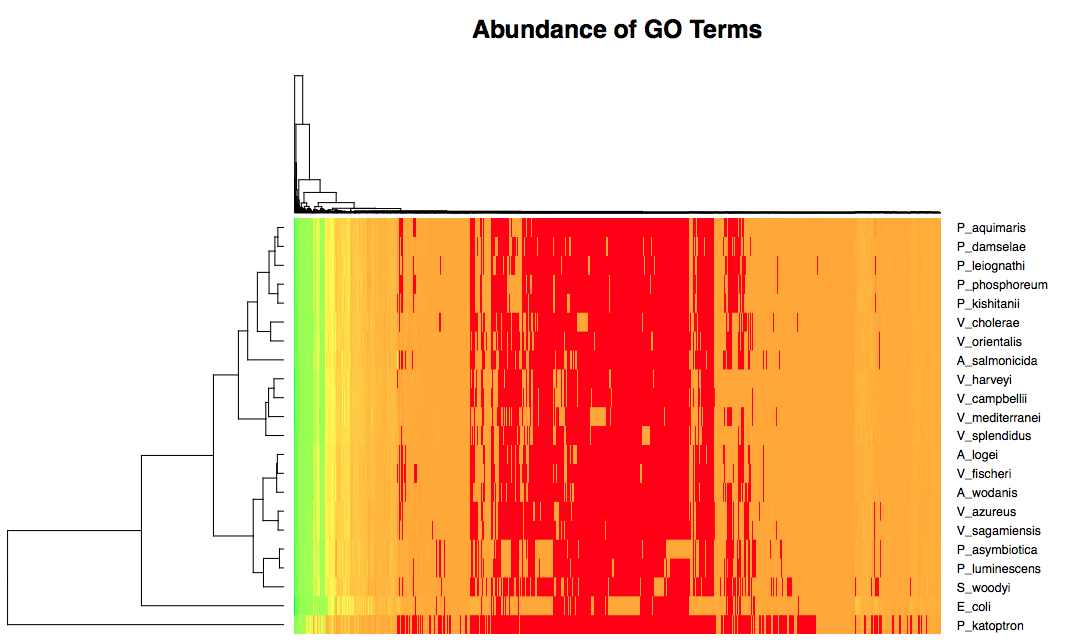
\includegraphics[width=\textwidth]{3.png}
\caption{Heat map of GO Terms from eggNOG-mapper for the 22 bacterial genomes. The X-axis lists over 6000 GO Terms, and the Y axis lists the species analyzed in this report. Red indicates GO terms that were absent, whereas green represents over 100 genes pertaining to a GO term.}
\centering
\label{fig3}
\end{figure}

The tree derived from NCBI taxonomy, showed \textit{Shewanella} and \textit{Photorhabdus} species to be the most distantly related to the \textit{Photobacterium}, \textit{Aliivibrio}, and \textit{Vibrio} genera, which are members of the \textit{Vibrionaceae} family \cite{t2}. Research by Urbanczyk et al. presents the hypothesis that \textit{Shewanella} and \textit{Photorhabdus} acquired the \textit{lux} genes from \textit{Aliivibrio} through horizontal transfer. If this hypothesis is correct, it would explain how these distantly related genera evolved the ability to bioluminesce \cite{t2}.

Figure \ref{fig3} was constructed using annotations from eggNOG-mapper, and is based on similarities between GO term sets of each prokaryotic species. In this tree, \textit{Candidatus photodesmus katoptron} appears to be the most distantly related. This differs from the organization of the tree based on NCBI taxonomy, in which \textit{S. woodyi} was most distantly related. \textit{Candidatus photodesmus katoptron} is a luminous symbiont of flashlight fish, and many of the functions required for sustaining life may be provided by the host \cite{24}. The nature of this specific interaction may differ greatly from the other symbiotic bioluminescent prokaryotes, which could result in the difference in functional distribution, and therefore GO term sets, between \textit{Candidatus photodesmus katoptron} and the other analyzed species. \textit{Candidatus photodesmus katoptron} has been found to be difficult to culture in a laboratory setting, due to it being an obligate symbiont and requiring the  stringent conditions of its host. These factors make the nature of this symbiotic relationship difficult to characterize and compare \cite{t3}. This result differs from the expected. It was initially expected that \textit{E. coli} would be the outgroup, as it does not exhibit bioluminescence or the respective \textit{lux} operon. However some strains of \textit{E. coli} are also involved in a mutually beneficial symbiotic relationship, as many of the other selected species are \cite{d9}.

Further comparison between the trees in figure \ref{fig1} and figure \ref{fig3} reveals slightly different branching schemes, which indicates that the bacteria’s evolutionary relationships does not exactly correlate with functional, metabolic similarities. The two \textit{Photorhabdus} species were seen to be more closely related to the \textit{E. coli} outgroup on the NCBI taxonomy tree, but on the GO term-derived tree \textit{Photorhabdus} was more closely grouped to other bioluminescent bacteria. In the phylogenetic tree derived from NCBI taxonomy, the genera \textit{Vibrio} and \textit{Aliivibrio} are found in very distinct groups, while in the tree derived from GO term similarity, species of these genera are intermixed, indicating overall functional similarities.

\begin{figure}[ht]
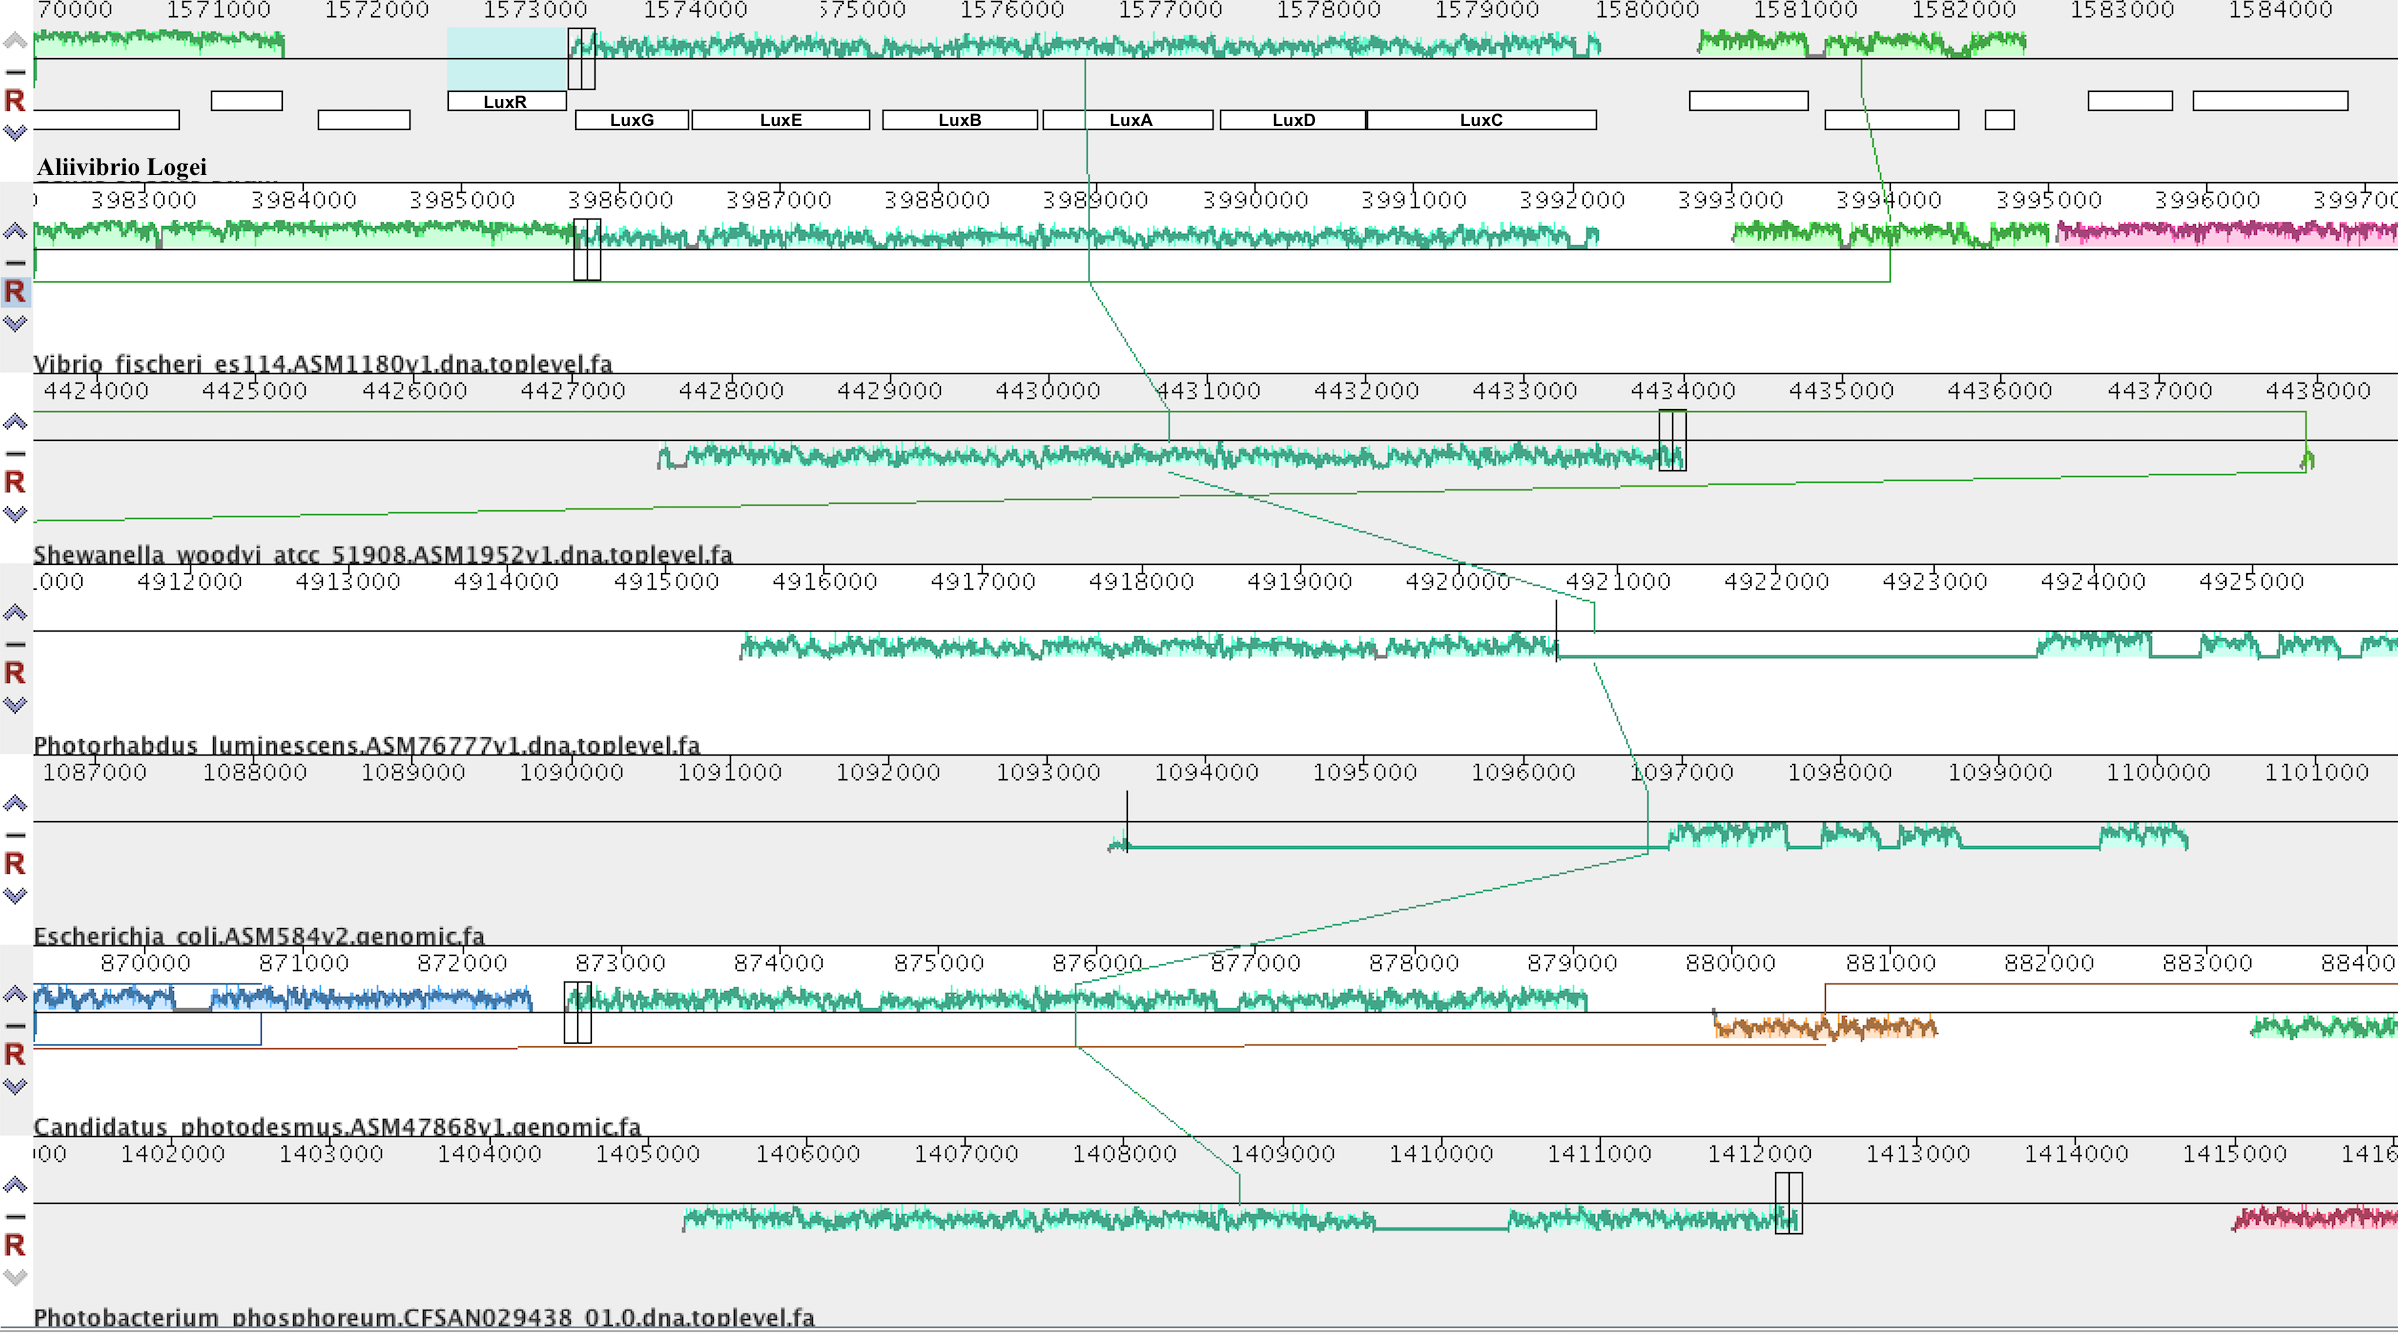
\includegraphics[width=\textwidth]{synteny.png}
\caption{Visualization of \textit{lux} operon synteny in 7 representative species. The \textit{luxCDABE} operon of \textit{A. logei} was mapped to \textit{A. fischeri}, \textit{S. woodyi}, \textit{P. luminescens}, \textit{E. coli}, \textit{Candidatus Photodesmus katoptron}, and \textit{P. phosphoreum}, and shows a high degree of synteny in this operon in most of the organisms.}
\centering
\label{fig4}
\end{figure}

The \textit{lux C, D, A, B,} and \textit{E} genes are known to make up the \textit{lux} operon, and were found to be present in the majority of analyzed species upon gene set comparison \cite{10}. A representative species from each genus analyzed in this project was selected for whole-genome synteny comparison, which revealed that the order of these \textit{lux} genes, and therefore the organization of the \textit{lux} operon, was conserved among the six bioluminescent genera. The position of the operon in each genome differs, but the high level of conservation of the operon’s structure implies functional importance of the \textit{lux} operon, which is shown in figure \ref{fig4}. The only species shown to have no sign of the operon was \textit{E. coli}, which was expected.  


\section*{Conclusions}

To summarize, prokaryotic bioluminescence pathways are not well understood. The \textit{lux} operon plays a crucial role in the pathway, with \textit{luxA} and \textit{luxB} encoding the heterodimeric luciferase protein. It is possible that eukaryotic luciferase proteins arose through convergent evolution, although further analysis is required to support this. The \textit{luxCDABE} operon displays syntenic gene order indicating functional importance of each of the components in the bioluminescence pathway. It appears that the \textit{Vibrio} genus employs a unique two component pathway involving \textit{Lux N, O, Q, R, U} genes to regulate bioluminescence. These genes do not appear to be highly represented in the other genera we analyzed. When comparing the branching schemes of the phylogenetic tree and and GO term tree, it was determined that functional relationships between species do not parallel the phylogenetic relationships. Branching of functional relationships is likely due to other factors such as specific symbiotic relationships. It is also thought that the bioluminescent capabilities of some genera, such as \textit{Shewanella} and \textit{Photorhabdus}, are most likely due to horizontal gene transfer from other bioluminescent species. Overall, bioluminescence has large functional importance in many species, multiple applications in molecular biology research, and possibly many other uses yet to be discovered.


\section*{Challenges}

The analyses performed for this project came with many challenges and complications. One limitation was the computational power of the devices used to carry out analyses, especially the genome annotations. Functional annotation of 22 prokaryotic genomes using pFastGO required over 40 hours of continuous analysis, which was made more manageable by dividing the analysis among four computers. The time-consuming nature of these genomic analyses limited the number of genomes that could be investigated.

The specific computational methods chosen for this project can make the task of interpreting derived results difficult. The use of different pipelines for genome annotation may yield different results, and some pipelines may be more effective at identifying and annotating every gene in the genome \cite{t4}. As a result of this limitation, there may be \textit{lux} genes or \textit{lux}-like genes present in the analyzed genomes which were not annotated by pfastGO. This lowers the confidence of the obtained results, as well as making it difficult to compare these results to those in the literature that were derived using alternate pipelines.

As bioluminescence is not well understood, all genes critical to this process may not have been identified and characterized. Bioluminescence has also been studied extensively in some species (ie. \textit{Aliivibrio fischeri}), but very little in others, which makes comparing bioluminescent pathways between species difficult, due to this sequencing bias.

\section*{Future Directions}

To further investigate bioluminescence pathways and their functional significance, more detailed analyses should be performed. The percentage of genes in each bacterial genome dedicated to bioluminescence and its related pathways could be investigated through construction of functional gene profiles. This would provide a better indication of how functionally important bioluminescence is to members of different genera. This is of specific interest in deep sea marine species where light acts as the major form a communication \cite{d10}. 

There appears to be potential involvement of \textit{lux}-like genes in the bioluminescence pathway. These genes should be investigated to determine how their sequences and functionality are similar or different from \textit{lux} genes. Specifically, species which have been observed to perform bioluminesce but do not appear to contain luciferase genes, such as \textit{luxA} or \textit{luxB} should be examined.

The genes and bioluminescence pathways are different in prokaryotes and eukaryotes. This project focuses on prokaryotic bioluminescence, but leaves the eukaryotic mechanisms to be investigated. Firefly luciferase is the most well-known eukaryotic luciferase, but the whole genome of the firefly has yet to be fully sequenced and assembled due to the abundance of highly variable repetitive elements \cite{t5}. Once the firefly genome information, as well as genome information of other bioluminescent eukaryotes is published, a comparative genomics analysis of these species would be informative. 

\newpage
\bibliographystyle{unsrt}
\bibliography{biol469.bib}

\end{document}
